\chapter{入力に0次ホールド機構を加えた連続時間システムのz変換}
    \section{背景}
        実用上、物理系をディジタル計算機で制御するために、連続系である制御対象と入力の間に「AD変換器」(0次ホールド回路+量子化器),「演算回路」,「DA変換器」(0次ホールド回路)が追加される。
        本節では、連続時間システムの入力に0次ホールド機構を追加したときのシステムの出力のうち、サンプリング時間の整数倍の時点に於いて出力が厳密に一致する離散時間システムのz変換を導出する。
    \section{主張}
        \renewcommand{\uH}{u_\text{H}}
        \newcommand{\ud}{u_\text{d}}
        \newcommand{\udd}{u_\text{dd}}
        \newcommand{\ydd}{y_\text{dd}}
        \newcommand{\hd}{h_\text{d}}
        \newcommand{\hdd}{h_\text{dd}}
        \newcommand{\Ud}{U_\text{d}}
        \newcommand{\Udd}{U_\text{dd}}
        \newcommand{\Hd}{H_\text{d}}
        \newcommand{\Hdd}{H_\text{dd}}
        \newcommand{\Ydd}{Y_\text{dd}}
        連続時間システムのインパルス応答を$h:\realNumbers\to\complexNumbers$とし、そのラプラス変換を$H:\complexNumbers\to\complexNumbers$とする。
        但しシステムは因果的である、すなわち$h(t)=0\;(t<0)$とする。
        入力信号をサンプリング周期$\Ts>0$で0次ホールドして与えるときの出力を$\yd:\realNumbers\to\complexNumbers$とする。
        このとき、システムのz領域の伝達関数は$(1-z^{-1})\Hdd(z)$となる。
        ここに$\Hdd(z)$は$H(s)/s$の逆ラプラス変換を周期$\Ts$でサンプリングして得られる離散時間信号のz変換である。
        つまり、このz領域の伝達関数の出力は$\Ts$の整数倍の時刻で連続時間システムの出力$\yd$と厳密に一致する。
        \begin{figure}[H]
            \centering
            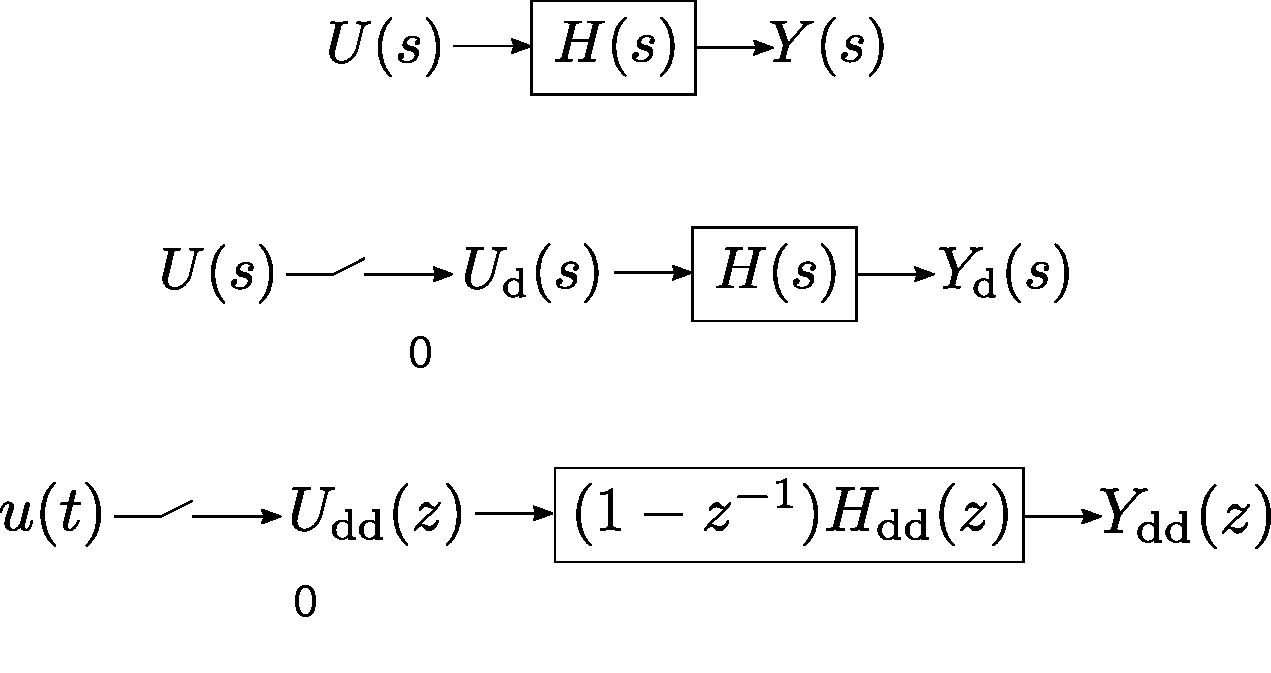
\includegraphics[keepaspectratio, scale=0.4]
            {\currfiledir/imgs/z-transform_with_0-order-hold_input.pdf}
            \caption{連続時間系と、入力に0次ホールドを付加した系}
        \end{figure}
    \section{導出}
        連続時間システムへの入力を$u:\realNumbers\to\complexNumbers$とする。
        但し$u(t)=0\;(t<0)$とする。
        周期$\Ts$で0次ホールドされた入力信号を$\ud:t\in\realNumbers\to u(\floor{t/\Ts}\Ts)$とする。
        Heavisideの単位ステップ関数を$\uH$とすると$\ud$は次式で表せる。
        \[ \ud(t) = \sum_{k=0}^\infty u(k\Ts)\left(\uH(t-k\Ts) - \uH(t-(k+1)\Ts)\right) \]
        これのラプラス変換を$U_\text{d}$とすると次式で表される。
        \[ \Ud(s) = \sum_{k=0}^\infty u(k\Ts)\NapierE^{-k\Ts s}\frac{1-\NapierE^{-\Ts s}}{s} \]
        これに対する出力$\yd$のラプラス変換を$\Yd$とすると、次式である。
        \begin{align*}
            \Yd(s) &= \sum_{k=0}^\infty u(k\Ts)\NapierE^{-k\Ts s}\frac{1-\NapierE^{-\Ts s}}{s}H(s) = \sum_{k=0}^\infty u(k\Ts)\NapierE^{-k\Ts s}\left(1-\NapierE^{-\Ts s}\right)\Hd(s) \\
            &\phantom{=} \text{where} \quad \Hd(s) \coloneqq H(s)/s
        \end{align*}
        $\Hd(s)$の逆ラプラス変換を$\hd$とすると、$\yd$は次式である。
        \[ \yd(t) = \sum_{k=0}^\infty u(k\Ts)(\hd(t-k\Ts)-\hd(t-(k+1)\Ts)) \]
        離散時間信号$\hdd,\ydd$を$\hdd:n\in\integers\mapsto \hd(n\Ts),\ydd:n\in\integers\mapsto \yd(n\Ts)$とすると$\ydd$は次式である。
        \begin{align*}
            \ydd(n) &= \yd(n\Ts) = \sum_{k=0}^\infty u(k\Ts)(\hd((n-k)\Ts)-\hd((n-k-1)\Ts)) \\
            &= \sum_{k=0}^\infty u(k\Ts)(\hdd(n-k)-\hdd(n-k-1))
        \end{align*}
        離散時間信号$\udd$を$\udd:n\in\integers\mapsto\ud(n\Ts)$で定義する。
        $\udd,\hdd,\ydd$のz変換をそれぞれ$\Udd,\Hdd,\Ydd$とすると次式を得る。
        \begin{align*}
            \Ydd(z) &= \sum_{n=0}^\infty \ydd(n) z^{-n} = \sum_{k=0}^\infty \ud(k\Ts) \sum_{n=0}^\infty ((\hdd(n-k)-\hdd(n-k-1))) z^{-n} \\
            &= \sum_{k=0}^\infty \ud(k\Ts)\left[z^{-k}\sum_{n=0}^\infty \hdd(n-k)z^{-(n-k)} - z^{-k-1}\sum_{n=0}^\infty \hdd(n-k-1)z^{-(n-k-1)}\right] \\
            &= \sum_{k=0}^\infty \ud(k\Ts)\left[z^{-k}\sum_{n=k}^\infty \hdd(n-k)z^{-(n-k)} - z^{-k-1}\sum_{n=k+1}^\infty \hdd(n-k-1)z^{-(n-k-1)}\right] \\
            &= \left(\sum_{k=0}^\infty \ud(k\Ts)z^{-k}\right)(1-z^{-1})\Hdd(z) = \Udd(z)(1-z^{-1})\Hdd(z)
        \end{align*}